\documentclass[10pt]{beamer}
\usepackage[utf8]{inputenc}
\usepackage[T1]{fontenc}
\usepackage[francais]{babel}
\usepackage{amsmath}
\usepackage{amssymb}
\usepackage{mathrsfs}
\usepackage{graphicx}

\usepackage{mathrsfs}
\usepackage{graphicx}
\usepackage{slashbox}
\usepackage{multirow}
\usepackage{algorithm,algorithmic}
\usepackage{pdfpages}
%\usepackage[top=2cm, bottom=2cm, left=2cm, right=2cm]{geometry}
%\usepackage[hmargin=2cm,vmargin=2cm,head=0.5cm,headsep=0pt,foot=0.5cm]{geometry}

\usetheme{Madrid}
\useoutertheme{split}
\usecolortheme{whale}

\newcommand{\xeon}{{\small \textsf{Xeon E5}}\xspace}
\newcommand{\altix}{{\small \textsf{Altix UV 2000}}\xspace}
\newcommand{\carma}{{\small \textsf{Carma}}\xspace}
\newcommand{\snowball}{{\small \textsf{Snowball}}\xspace}
\newcommand{\mppa}{{\small \textsf{MPPA-256}}\xspace}

%\usecolortheme{seagull}
\setbeamercolor*{titlelike}{parent=structure}



% logo of my university
%\titlegraphic{
 %   
\includegraphics[width=1.2cm]{images/logo_ird}\hspace*{1cm}~%
    %
\includegraphics[width=1.2cm]{images/logo_ummisco}\hspace*{1cm}~%
    %
\includegraphics[width=1.2cm]{images/logo_uy1}\hspace*{1cm}~%
  %  
\includegraphics[width=1.2cm]{images/logo_lirima}\hspace*{1cm}~%
   % 
\includegraphics[width=1.2cm]{images/logo_lig}\hspace*{1cm}~%
    %
\includegraphics[width=1.2cm]{images/logo_inria}\hspace*{1cm}~%
%}
\title[Titre du Mémoire]{DSL pour la fouille des réseaux sociaux sur des plates-formes multi-coeurs}
\author[Nom1, Nom2, Nom3]{Thomas Messi Nguélé\\ \ \\ sous la co-direction de\\ \ \\ Pr Jean-François Méhaut, Pr Maurice Tchuente}
\expandafter\def\expandafter\insertshorttitle\expandafter{%
  \insertshorttitle\hfill%
  %\insertframenumber\,/\,\inserttotalframenumber
  }

%\setbeameroption{hide notes}
%\setbeameroption{show notes on second screen}
%\setbeameroption{show notes on second screen}
%\setbeameroption{show only notes}
\begin{document}

\begin{frame}
%\titlepage

%\setbeamercolor{background canvas}{bg=}
%
\includepdf[pages={1}]{couverture_presentation_messi.pdf}
%\vspace*{-1pt}
\makebox[\linewidth]{
\includegraphics[page={1},width=\paperwidth]{couverture_presentation_messi.pdf}}

\end{frame}
%\AtBeginSection[]{
%}

\section{Introduction}
\subsection{Contexte}
\begin{frame}
\frametitle{Réseau social}
%\begin{block}{}
 \begin{itemize}
 \item ensemble d'entités (individus, organisations,...) interconnectées par des liens (amitié, échanges de messages,...).
 \item modélisation à l'aide des \textbf{graphes}
	\begin{itemize}
	 \item \textbf{très grand nombre de noeuds}, facebook 1.15 milliard, YouTube 1 milliard, Twitter 200 millions
	 \item \textbf{faible densité de liens}, un noeud est lié en moyenne à 150 autres noeuds.
	\end{itemize}
 \item Exemple: le réseau des chercheurs de physique quantique (Quant-ph) \cite{quant-ph} a 1060 n\oe uds et 1044 arêtes;
	\begin{itemize}
	 \item arêtes possibles: \textbf{561270}, soit une densité de \textbf{0.2\%};
	 \item katz \cite{articlekatz} ou rules  \cite{vanessaMasterThesis} tourne sur \textbf{560226} soit \textbf{99.8\%}.
	 \item \textbf{\textcolor{red}{Plusieurs heures d'exécution en mode séquentiel}}.
	\end{itemize}
\end{itemize}
%\end{block}
\end{frame}

\begin{frame}
\frametitle{Comment réduire le temps d'exécution?}
%\begin{block}{}
\begin{itemize}
 \item Usage des architectures multi/many-c\oe urs.
 \item Mais, difficultés pour écrire des programmes parallèles efficaces et tirant profit de la multitude des c\oe urs disponibles \cite{articlemppa,articlemppacri}.
 \begin{itemize}
  \item Écriture du code de bas niveau spécifique à la plate-forme.
 \end{itemize}
\end{itemize}
%\end{block}
\end{frame}
\subsection{Problème}
\begin{frame}
\frametitle{Problème}
%\begin{block}{}
\begin{itemize}
 \item Comment permettre aux chercheurs (algorithmiciens) de la fouille des réseaux d'écrire \textbf{facilement} et \textbf{efficacement} des \textbf{programmes parallèles} s'exécutant sur des multi/many-c\oe urs?
 \item Deux étapes proposées:
    \begin{enumerate}
      \item Étude des possibilités des architectures multi/many-coeurs.
      \item Conception et réalisation d'un langage dédié (\textit{Domain Specific Langage}, \textbf{DSL}).
    \end{enumerate}
\end{itemize}
%\end{block}
\end{frame}
\subsection{Plan}
\begin{frame}{Plan}
    \tableofcontents[sections={2-8},hideothersubsections]
\end{frame}
% ----------------------------------------Evolution des architectures---------------------------------------
\section{Étude des possibilités des architectures multi/many-c\oe urs}
\subsection{Présentation des architectures}
\begin{frame}
\frametitle{Xeon E5 d'Intel}
  \begin{columns}[T]
    \begin{column}{.55\textwidth}
    \begin{block}{Vue simplifiée du \xeon}
    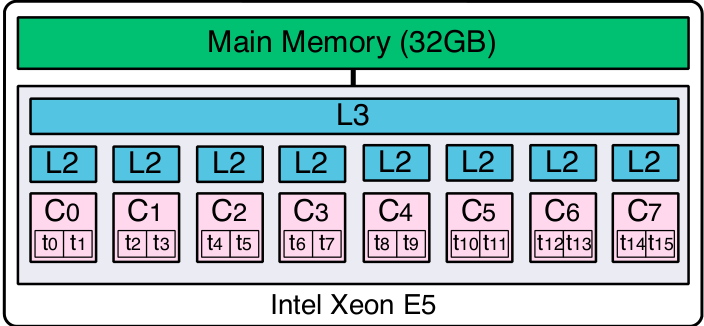
\includegraphics[scale=0.27]{figures/xeon}
    \end{block}
    \end{column}
    \begin{column}{.4\textwidth}
     \begin{block}{Caractéristiques}
      \begin{itemize}
       \item processeur généraliste
       \item 8 coeurs, supportant l'hyperthreading;
       \item 3 niveaux de cache
       \item 2.4GHZ
       \item 68.6 watt
      \end{itemize}
     \end{block}
    \end{column}
  \end{columns}
\end{frame}

\begin{frame}
\frametitle{MPPA-256 de Kalray}
  \begin{columns}[T]
    \begin{column}{.55\textwidth}
    \begin{block}{Vue simplifiée du \mppa}
    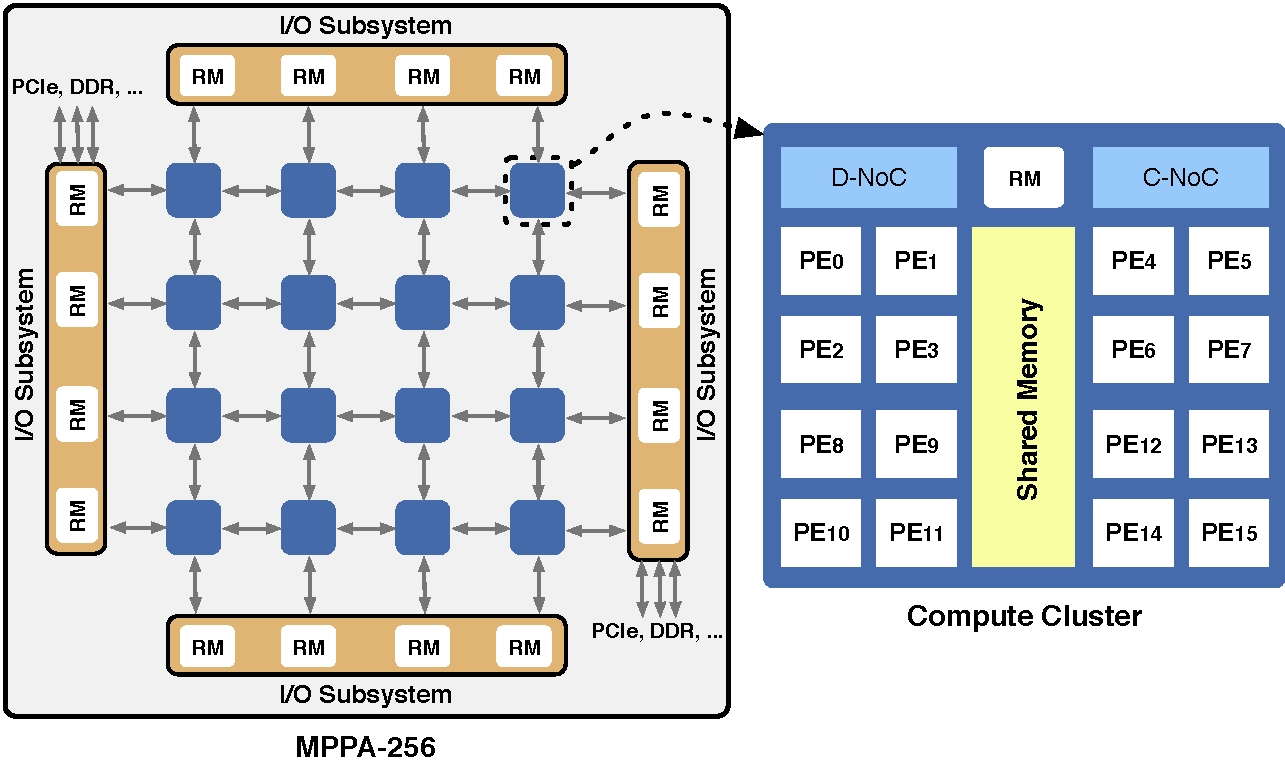
\includegraphics[scale=0.26]{figures/mppa_overall}
    \end{block}
    \end{column}
    \begin{column}{.4\textwidth}
     \begin{block}{Caractéristiques}
      \begin{itemize}
       \item 16 clusters de calcul
       \item 16 coeurs par cluster, soit en tout 256 coeurs
       \item 2 Mo de RAM par cluster
       \item 400 MHZ
       \item 10.7 watt
      \end{itemize}
     \end{block}
    \end{column}
  \end{columns}
\end{frame}

\subsection{Le TSP}
\begin{frame}
\frametitle{Le TSP}
  \begin{columns}[T]
    \begin{column}{.55\textwidth}
    \begin{block}{Problème du voyageur de commerce}
% Your image included here
    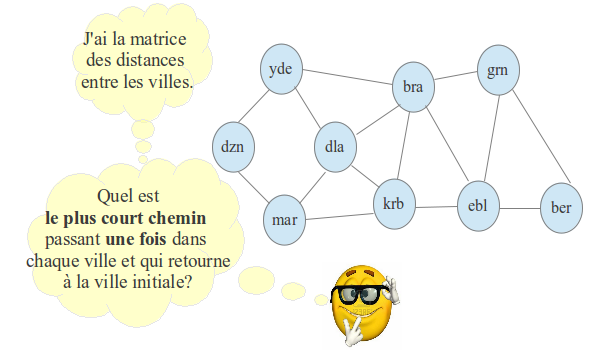
\includegraphics[scale=0.32]{figures/TSP_problem.png}
    \end{block}
    \end{column}
    \begin{column}{.4\textwidth}
     \begin{block}{À propos du TSP}
      \begin{itemize}
       \item L'itinéraire le plus court
       \item Problème NP-complet
       \item Influencé par le dégré de parallélisme
      \end{itemize}
     \end{block}
    \end{column}
  \end{columns}
\end{frame}
\subsection{Approche de résolution du TSP}
\begin{frame}
\frametitle{}
\begin{columns}[T]
    \begin{column}{.49\textwidth}
    \begin{block}{Mét. de séparation et d'évaluation}
	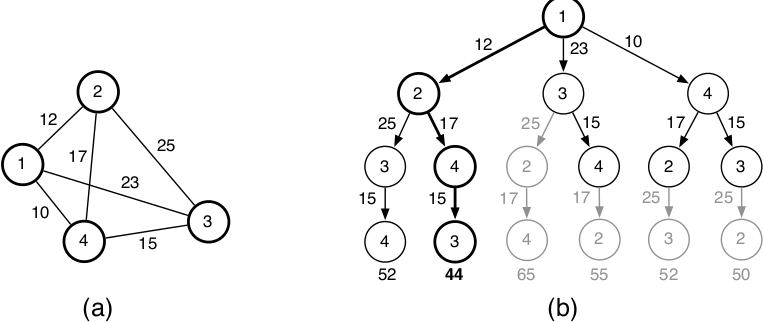
\includegraphics[scale=0.22]{images/approche_tsp.png}
    \end{block} 
    \end{column}
    \begin{column}{.4\textwidth}
     \begin{block}{}
      \begin{itemize}
        \item Chemins à explorer plus courts que le meilleur chemin déjà rencontré,
        \item complexité dans le pire des cas $O(n!)$.
      \end{itemize}
     \end{block}
    \end{column}
  \end{columns}
\begin{block}{}
   \begin{enumerate}
	   \item Algorithme séquentiel: mise à jour séquentielle du chemin minimal.
	   \item Algorithme multi-threadé: présence d'une file de tâches, mise à jour parallèle.
	   \item Algorithme distribué: mise à jour diffusée dans tous les postes de calcul.
  \end{enumerate}
\end{block}
\end{frame}

\subsection[Adaptation à un many-c\oe urs]{Adaptation du TSP à une Plate-forme Many-coeurs}
\begin{frame}
\frametitle{Adaptation sur \mppa}
%\begin{block}{}
 \begin{itemize}
  \item Solution multi-threadée pour les deux plates-formes, $min\_path$ comme variable partagée.
  \item Inappropriée pour le \mppa, caches non cohérents.
  \item Correction avec les inscructions spécifiques à la plate-forme.
 \end{itemize}
%\end{block}
\end{frame}
\subsection{Quelques résultats de l'étude}
\begin{frame}
\begin{columns}[T]
    \begin{column}{.47\textwidth}
    \begin{block}{\mppa \ vs \xeon}
	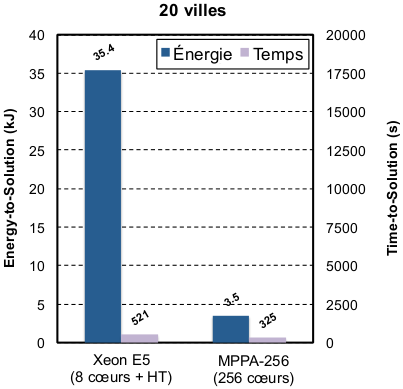
\includegraphics[scale=0.4]{figures/en_ti_solution}
    \end{block}
    \end{column}
    \begin{column}{.5\textwidth}
     \begin{block}{Observations}
      \begin{itemize}
       \item le TSP s'exécute 1,6x plus vite sur \mppa
       \item \mppa \ réduit la conso. de \xeon \ de 90\%
      \end{itemize}
     \end{block}
      \begin{block}{Expli.: mise en oeuvre du TSP}
	\begin{itemize}
	\item peu d'échanges de messages entre les postes,
	\item diffusion implémentée avec les messages asynchrones à travers le NOC,
	\item donc absence de contention.
	\end{itemize}
      \end{block}
    \end{column}
  \end{columns}
  Many-c\oe urs comme \mppa \ \textbf{\textcolor{green}{donnent de très bons résultats}}, mais \textcolor{red}{nécessitent beaucoup d'efforts} de la part du programmeur.
\end{frame}

% -----------------------Fouille des réseaux sociaux-----------------------------------------
\section{Fouilles des réseaux sociaux}
\subsection{Généralités}
\begin{frame}% [allowframebreaks=0.50]
\frametitle{}
\begin{columns}[T]
    \begin{column}{.895\textwidth}
    \begin{block}{Tâches dans la fouille des réseaux sociaux}
    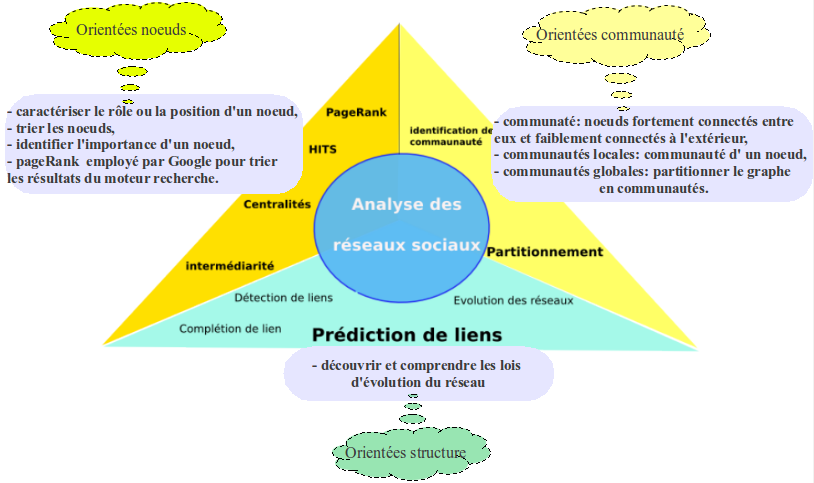
\includegraphics[scale=0.38]{images/tache_fouille_donnees_2.png}
    \end{block}
    \end{column}
  \end{columns}
\end{frame}

% ----------------------------------------Présentation du DSL-------------------------------------------------------
\section{DSL pour la fouille des réseaux Sociaux}
\subsection{Généralités sur les DSLs}
\begin{frame}
\frametitle{Généralités sur les DSL}

%\begin{block}{}
\begin{itemize}
       \item Langage de programmation conçu pour un domaine précis
	\item Exemples: HTML, SQL, YACC, ...
      \end{itemize}
\begin{itemize}
 \item Deux approches d'implémentation \cite{dsloverview}:
      \begin{enumerate}
      \item DSL externe ou "stand alone";
      \item DSL interne ou embarqué.
      \end{enumerate}
 \item Ici, l'approche embarquée avec Erlang comme langage hôte.
\end{itemize}
%\end{block}
\end{frame}

\subsection{Présentation du DSL}
\begin{frame}% [allowframebreaks=0.50]
\frametitle{}
\begin{columns}[T]
    \begin{column}{.46\textwidth}
      \begin{block}{Présentation du DSL}
    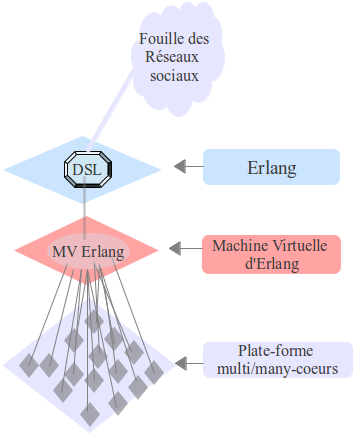
\includegraphics[scale=0.445]{images/presentationDuDSL.png}
    \end{block}
    \end{column}
    \begin{column}{.48\textwidth}
    \begin{block}{}
      \begin{itemize}
       \item[*] DSL est embarqué dans Erlang
       \item[*] faciliter la programmation parallèle sur des multi/many-c\oe urs,
      \end{itemize}
    \end{block}
    \begin{block}{}
      \begin{itemize}
       \item[-] types de base d'Erlang restent utilisés,
       \item[-] 3 principaux types: graphe, arête et noeud (à partir de digraph),
      \end{itemize}
    \end{block}
    %\begin{block}{}
      \begin{itemize}
       \item Plusieurs primitives utilisées dans la fouille des réseaux
       \item création d'objets graphe, manipulation (n\oe uds, arêtes), ...
       \item DSL Green-Marl, les travaux de l'equipe (E. Viennet, B. Kaledjé, V. Kamga, M. Tchuente).
      \end{itemize}
    %\end{block}
    \end{column}
  \end{columns}
\end{frame}
\subsection{Parallélisme dans le DSL}
\begin{frame}
\frametitle{}
\begin{block}{Parallélisme dans le DSL}
 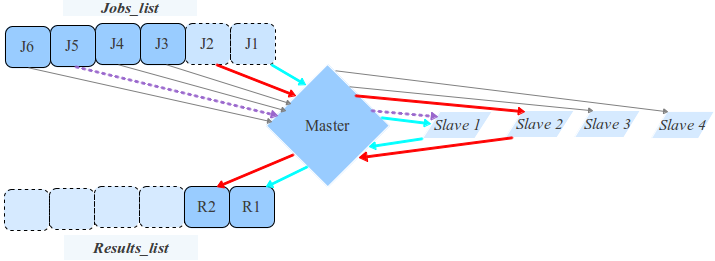
\includegraphics[scale=0.46]{images/dsl_parallelism.png}
\end{block}
\begin{block}{}
 \begin{itemize}
  \item parallel\_op permet d'écrire facilement des programmes parallèles,
  \item le maître a une liste de job et une liste des resultats,
  \item le maitre attribue des jobs aux esclaves et range les resultats des esclaves,
  \item approche implémentée dans \cite{articledisnet}.
 \end{itemize}

\end{block}
\end{frame}
% ----------------------------------------Analyse des performances----------------------------------------------
\section{Étude de cas: implémentation du score de Katz}
\subsection{Le score de Katz}
\begin{frame}
\begin{block}{Le score de Katz \cite{articlekatz,articledavidjon}}
    \begin{itemize}
     \item Mesure de similarité basée sur les distances entre les n\oe uds.
     \item $katz\_score(x,y) = \sum_{l=1}^{\infty}(\beta^{l}.|paths_{x,y}^{<l>}|)$
    \end{itemize}
    \end{block}
\begin{block}{Algorithme}
{\fontsize{10}{10}\selectfont
\begin{algorithmic}[1]
\STATE \textbf{katz\_score}($x,y,\beta,max\_l,G$)
\STATE $ktz\_score \leftarrow 0.0$
\FOR {$l=1$ to $max\_l$}
   \STATE \label{appel_paths_leaves}$leaves\_list \leftarrow \textbf{paths\_leaves}(x,y,l,0,G)$
   \STATE \label{appel_occurence_count} $nb\_path\_l \leftarrow occurence\_count(y, leaves\_list)$
   \STATE  $ktz\_score \leftarrow ktz\_score + \beta^l * nb\_path\_l$
\ENDFOR
\RETURN $ktz\_score$
\end{algorithmic}
}
\end{block}
\end{frame}

\begin{frame}
\begin{columns}[T]
    \begin{column}{.55\textwidth}
    \begin{block}{Calcul du nombre de chemins}
      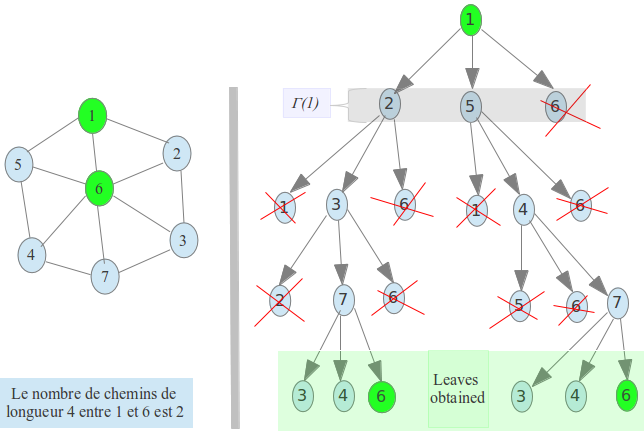
\includegraphics[scale=0.29]{images/exemple_d_execution.png}
    \end{block}
    \end{column}
    \begin{column}{.4\textwidth}
    \begin{block}{Commentaires}
      \begin{itemize}
       \item x=1, y=6, l=4.
       \item Arbre de racine x et de hauteur l.
       \item Nombre de y en feuilles: 2.
      \end{itemize}

    \end{block}
    \end{column}
  \end{columns}
\end{frame}
\subsection{Implémentation du score de katz}
\begin{frame}% [allowframebreaks=0.50]
\frametitle{}
\begin{exampleblock}{Implémentation avec le DSL}
      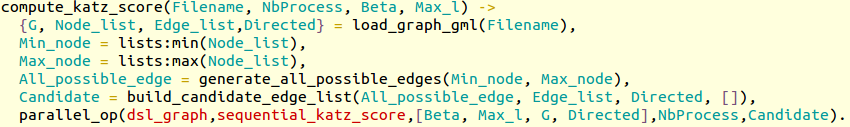
\includegraphics[scale=0.405]{images/exempleDeCodeDSL.png}
\end{exampleblock}
\begin{itemize}
 \item Moins d'effort à fournir.
\end{itemize}

\begin{block}{Nombre de lignes de code}
 \begin{center}
\begin{table}[h]
 \begin{tabular}{|c|c|c|c|c|c|}
   \hline
   Langages		  &C	&Java	&Python	&Erlang	&DSL\\
    \hline
   Nombre de ligne de code&944	&462	&284	&274	&30 \\
    \hline
  \end{tabular}
 \end{table}
\end{center}
\end{block}
\begin{itemize}
 \item Le DSL a \textbf{moins de lignes de code} que les autres langages.
\end{itemize}
\end{frame}

\subsection{Résultats sur les machines spécialisées au HPC}
\begin{frame}% [allowframebreaks=0.50]
\frametitle{}
\begin{block}{Évolution du temps d'exécution sur Numa32}
 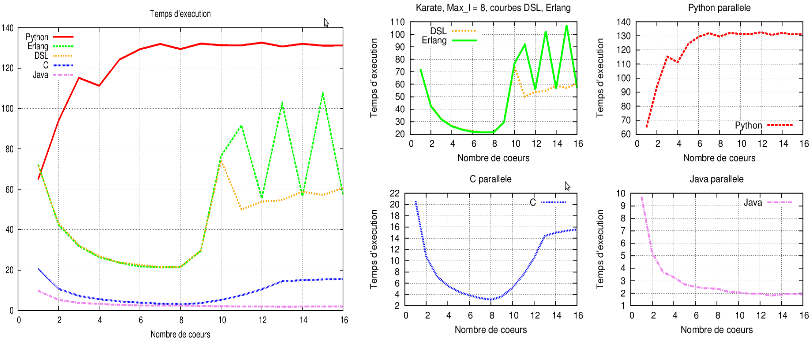
\includegraphics[scale=0.425]{images/kar_idr_time}
\end{block}
%\begin{block}{Commentaires}
 \begin{itemize}
  \item Diminution du temps d'exécution en fonction du nombre de c\oe urs.
  \item À  partir de 9 c\oe urs, le temps d'exécion augmente.
 \end{itemize}

%\end{block}
\end{frame}
\begin{frame}% [allowframebreaks=0.50]
\frametitle{}
\begin{columns}[T]
    \begin{column}{.65\textwidth}
      \begin{block}{Gains de parallélisme}
	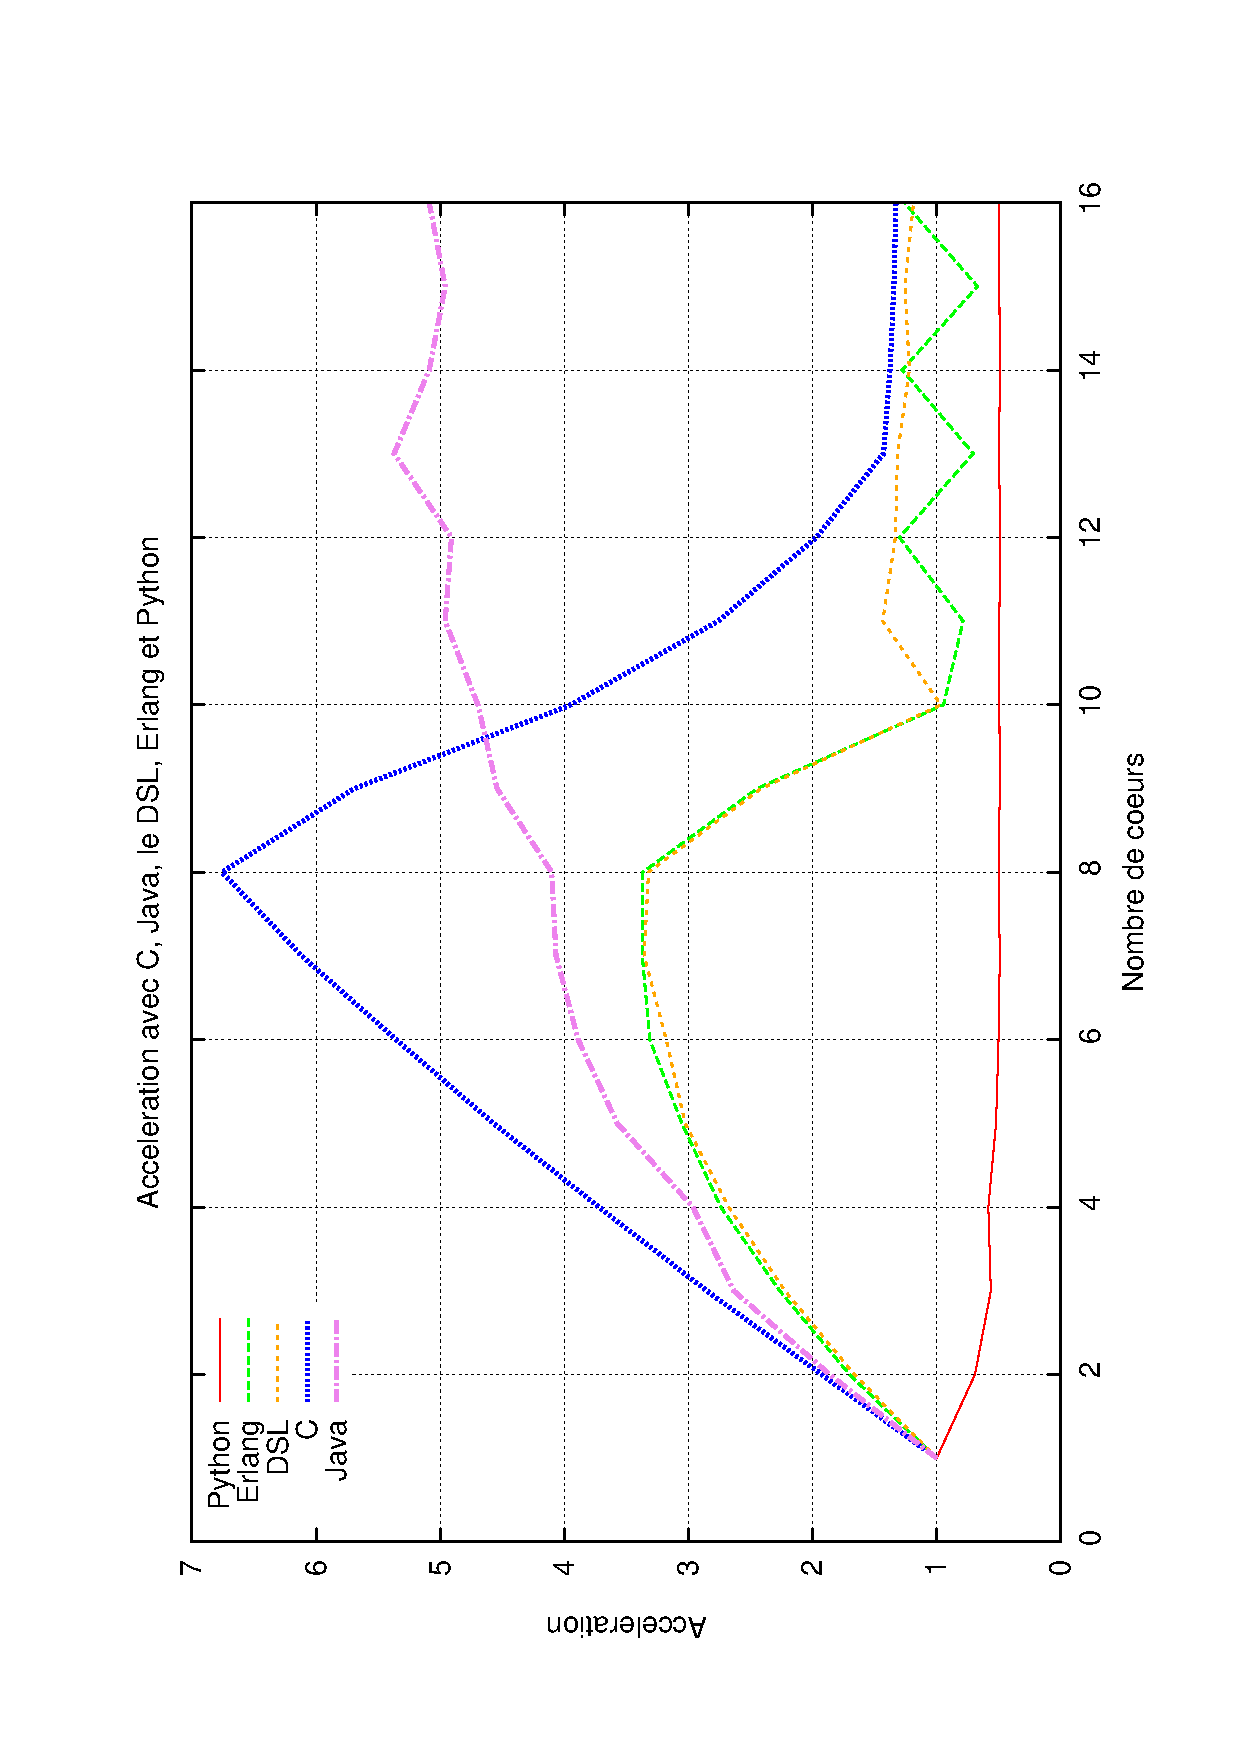
\includegraphics[scale=0.24]{images/kar_idro_speedup_same_scale}
      \end{block}
    \end{column}
    \begin{column}{.3\textwidth}
 %   \begin{block}{Commentaires}
      \begin{itemize}
       \item Accélération croissante jusqu'à 8 c\oe urs.
       \item Même accélération entre DSL et Erlang jusqu'à 8 c\oe urs
      \end{itemize}

  %  \end{block}
    \end{column}
  \end{columns}
\end{frame}
% -------------------Conclusion et perspectives-----------------------------------------------
\section{Conclusion et perspectives}
\begin{frame}% [allowframebreaks=0.50]
\frametitle{}
\begin{block}{Conclusion}
\begin{itemize}
 \item Objectif: \textbf{faciliter} la \textbf{programmation parallèle} des algorithmes de \textbf{fouille des réseaux sociaux} sur des plates-formes multi/many-coeurs.
 \item Contributions:
 \begin{enumerate}
  \item Étude des possibilités des architectures multi/many-coeurs.
	\begin{itemize}
              \item Très bonnes performances, 
              \item mais nécessitent beaucoup d'efforts.
        \end{itemize}
  \item DSL pour la fouille des réseaux sociaux.
	\begin{itemize}
              \item Facilité assurée,
              \item performance limitée par le langage hôte.
        \end{itemize}
 \end{enumerate}
\end{itemize} 
\end{block}

\begin{block}{Perspectives}
 \begin{itemize}
  \item DSL version stand-alone
  \item Gestion fine de l'allocation des threads
  \item Inclure d'autres applications et d'autres architectures dans l'étude des défis de programmation.
\end{itemize}
\end{block}

\end{frame}



\begin{frame}% [allowframebreaks=0.50]
\frametitle{}

    %
\includegraphics[scale=0.43]{images/merciDeVotreAttention}
    
\includegraphics[scale=0.43]{images/merci_de_votre_attention}
\end{frame}

\bibliographystyle{plain} % Le style est mis entre accolades.

\bibliography{bibli} % mon fichier de base de données s'appelle bibli.bib

\end{document}
